\documentclass{sprawozdanie-agh}

\usepackage{float}
\usepackage[utf8]{inputenc}
\usepackage{matlab-prettifier}
\usepackage{siunitx}
\usepackage{booktabs,caption,ragged2e}

\makeatletter

% ========= Początek Dokumentu ========= 
\begin{document}
% ========= Strona tytułowa ========= 
\przedmiot{Teoria Sterowania II: Ćwiczenia Laboratoryjne}
\tytul{Wytyczne dla Ćwiczenia 5}
\podtytul{Kryterium Koła i~Kryterium Popova}
\kierunek{Automatyke i~Robotyka}
\autor{Dariusz Cieślar, Maciej Różewicz}
\data{Kraków, \today}

\stronatytulowa{}
% ========= Treść Właściwa =========
\section{Cel ćwiczenia}
Celem ćwiczenia jest zapoznanie się z~dwoma kryteriami badania stabilności: kryterium Popova i~kryterium koła.
Obydwa służą do badania globalnej asymptotycznej stabilności tzw. układów Lurie.
Oparte są one na badaniu charakterystyki częstotliwościowej części liniowej
układu, podobnie jak w~kryterium Nyquista.
Jednak pozwalają na rozpatrywanie znacznie szerszej klasy sterowań/części nieliniowych, które mogą być nie tylko nieliniowe i~niestacjonarne, ale nawet niejednoznaczne.

%%%%%%%%%%%%%%%%%%%%%%%%%%%%%%%%%%%%%%%%%%%%%%%%%%%%%%%%%%%
\section{Przebieg ćwiczenia}
Dla każdego z~podanych systemów: \ref{sec:system_1}, \ref{sec:system_2}
i~\ref{sec:system_3} należy w trakcie ćwiczenia wykonać następujące kroki:
\begin{description}
    \item [Krok 1] Zweryfikować czy dla danego systemu można stosować kryterium Popova.
    \item [Krok 2] Jeśli tak, to wyznaczyć charakterystykę Popova. Jeśli nie
    sprawdzić czy można dokonać "wirtualnej" transformacji układu, która pozwoli
    na zastosowanie kryterium Popova i~wyznaczyć charakterystykę Popova dla
    układu po transformacji.
    \item [Krok 3] Wyznaczyć charakterystykę prostą Popova (jeśli można stosować
    kryterium Popova) zapewniającą jak największy sektor Popova.
    \item [Krok 4] Sprawdzić symulacyjnie dla zadanej nieliniowości czy układ
    jest stabilny dla wyznaczonego sektora Popova.
    \item [Krok 5] Zweryfikować czy można stosować kryterium koła.
    \item [Krok 6] Jeśli tak, to wyznaczyć charakterystykę Nyquista. Jeśli nie
    sprawdzić czy można dokonać "wirtualnej" transformacji układu, która pozwoli
    na zastosowanie kryterium koła i~wyznaczyć charakterystykę Nyquista dla
    układu po transformacji.
    \item [Krok 7] Wyznaczyć "koło" dla kryterium koła zapewniające jak
    największy sektor dopuszczalny z~kryterium koła.
    \item [Krok 8] Sprawdzić symulacyjnie dla zadanej nieliniowości czy układ
    jest stabilny dla wyznaczonego sektora dopuszczalnego z~kryterium koła.
    \item [Krok 9] Porównać wyniki z~obydwu kryteriów - porównać sektory Popova
    i~dopuszczalny z~kryterium koła.
\end{description}
Wynik każdego kroku należy umieścić w sprawozdaniu.

    %======================================================
    \subsection{System 1}\label{sec:system_1}
    Wyznaczyć największy sektor dopuszczalny w~kryterium Popova i~kryterium koła dla układu opisanego transmitancją (\ref{eq:system_1}) oraz nieliniowym elementem $\varphi(\cdot)$.% przedstawionych na rysunku (\ref{fig:zad_1}).
    \begin{equation}
        \label{eq:system_1}
        G_{1}(s) = \frac{4(1-5s)}{(1+3s)(1+2s)}
    \end{equation}
    Do sprawdzenia symulacyjnego proszę użyć następujących funkcji:
    \begin{itemize}
        \item $u = ky$ - gdzie $k$ jest dobrane jako:
        \begin{itemize}
            \item $k_{max}$ - największa wartość $k$ dla której charakterystyka
            elementu $\varphi(\cdot)$ mieści się w~sektorze Popova/koła,
            \item $k_{min}$ - najmniejsza wartość $k$ dla której charakterystyka
            elementu $\varphi(\cdot)$ mieści się w~sektorze Popova/koła,
            \item $\frac{1}{2}(k_{max} + k_{min})$,
        \end{itemize}
        \item $u = \frac{1}{2}k_{max}y(\sin{y} + 1)$.
    \end{itemize}

    %======================================================
    \subsection{System 2}\label{sec:system_2}
    Dany jest system dynamiczny:
    \begin{equation}
        \begin{array}{l}
            \dot{x} = Ax + bu\\
            y = c^{T}x 
        \end{array}
    \end{equation}
    gdzie:
    \begin{equation}
        A
        =
        \left[
        \begin{array}{rrr}
            -2 & 1 & 0\\
            -1 & 0 & 1\\
            -1 & 0 & 0
        \end{array}
        \right],\,
        b
        =
        \left[
        \begin{array}{r}
            -1\\
            0\\
            0
        \end{array}
        \right],\,
        c^{T}
        =
        \left[
        \begin{array}{ccc}
            1 & 0 & 0
        \end{array}
        \right].
    \end{equation}
    System ten objęto ujemnym sprzężeniem zwrotnym za pomocą nieliniowego, statycznego, stacjonarnego elementu o~charakterystyce:
    \begin{equation}
        u = M \arctan{y},\,M>0.
    \end{equation}
    Określić możliwie największą wartość parametru $M$, przy której charakterystyka elementu nieliniowego mieści się jeszcze w~sektorze Popova oraz sektorze dopuszczalnym dla kryterium koła.

    %======================================================
    \subsection{System 3}\label{sec:system_3}
    Zbadać asymptotyczną stabilność globalną układu regulacji przedstawionego na rysunku (\ref{fig:zad3}).
    Zakładamy, że w~układzie może występować dozwolony element nieliniowy o~charakterystyce $u = \varphi(y)$ spełniającej warunek $0 \leq y\varphi(y) \leq Ly^2$, dla $L = \frac{1}{2}$ i~$L = 2$.
    \begin{figure}[H]
        \centering
        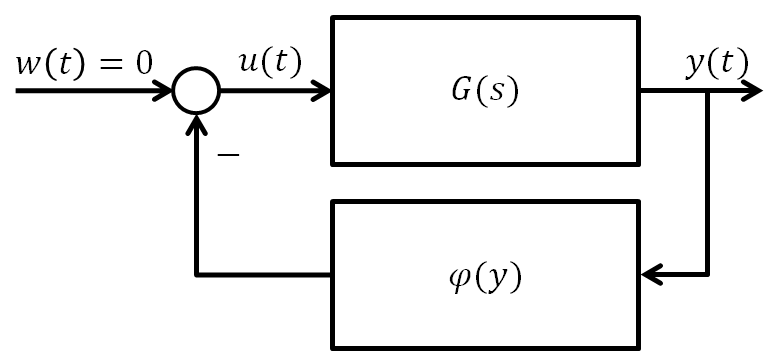
\includegraphics[width=0.5\linewidth]{fig/zad3.PNG}
        \caption{Układ dla zadania 3.}
        \label{fig:zad3}
    \end{figure}
    Gdzie transmitancja wynosi:
    \[
        G(s) = \frac{s^2+s+1}{s^4 + 2s^3 + s^2 + s + 1}
    \]
    Sprawdzić symulacyjnie dla nieliniowości dobranych jak w systemie \ref{eq:system_1}.

\end{document}
